\item \points{33} {\bf Semi-supervised EM}

\def\zsi{z^{(i)}}
\def\xsi{x^{(i)}}

Expectation Maximization (EM) is a classical algorithm for unsupervised learning (\emph{i.e.,} learning with hidden or latent variables). In this problem we will explore one of the ways in which the EM algorithm can be adapted to the semi-supervised setting, where we have some labelled examples along with unlabelled examples.

In the standard unsupervised setting, we have $\nexp \in \mathbb{N}$ unlabelled examples $\{x^{(1)},\ldots,x^{(\nexp)}\}$. We wish to learn the parameters of $p(x,z;\theta)$ from the data, but $\zsi$'s are not observed. The classical EM algorithm is designed for this very purpose, where we maximize the intractable $p(x;\theta)$ indirectly by iteratively performing the E-step and M-step, each time maximizing a tractable lower bound of $p(x;\theta)$. Our objective can be concretely written as:

\begin{align*}
    \ell_{\text{unsup}}(\theta) &= \sum_{i=1}^\nexp \log p(\xsi;\theta) \\
    &= \sum_{i=1}^\nexp \log \sum_{\zsi} p(\xsi,\zsi;\theta)
\end{align*}


Now, we will attempt to construct an extension of EM to the semi-supervised setting. Let us suppose we have an \emph{additional} $\tilde{\nexp} \in \mathbb{N}$ labelled examples $\{(\tilde{x}^{(1)},\tilde{z}^{(1)}),\ldots,(\tilde{x}^{(\tilde{\nexp})},\tilde{z}^{(\tilde{\nexp})})\}$ where both $x$ and $z$ are observed. We want to simultaneously maximize the marginal likelihood of the parameters using the unlabelled examples, and full likelihood of the parameters using the labelled examples, by optimizing their weighted sum (with some hyperparameter $\alpha$). More concretely, our semi-supervised objective $\ell_\text{semi-sup}(\theta)$ can be written as:
%
\begin{align*}
    \ell_\text{sup}(\theta) &= \sum_{i=1}^{\tilde{\nexp}} \log p(\tilde{x}^{(i)},\tilde{z}^{(i)};\theta) \\
    \ell_{\text{semi-sup}}(\theta) &= \ell_\text{unsup}(\theta) + \alpha \ell_\text{sup}(\theta)
\end{align*}
%
We can derive the EM steps for the semi-supervised setting using the same approach and steps as before. You are \emph{strongly encouraged} to show to yourself (no need to include in the write-up) that we end up with:

\subsubsection*{E-step (semi-supervised)}

For each $i \in \{1,\ldots,\nexp\}$, set
\begin{align*}
    Q_i^{(t)}(\zsi) := p(\zsi|\xsi;\theta^{(t)})
\end{align*}

\subsubsection*{M-step (semi-supervised)}

\begin{align*}
    \theta^{(t+1)} &:= \arg\max_\theta\left[ \sum_{i=1}^\nexp\left( \sum_{\zsi} Q^{(t)}_i(\zsi) \log \frac{ p(\xsi, \zsi;\theta) }{ Q^{(t)}_i(\zsi)}\right)  + \alpha \left(\sum_{i=1}^{\tilde{\nexp}} \log p(\tilde{x}^{(i)},\tilde{z}^{(i)};\theta)\right)\right]
\end{align*}

\begin{enumerate}
  \item\subquestionpointswritten{5}
\textbf{Convergence.}
First we will show that this algorithm eventually converges. In order to prove this, it is sufficient to show that our semi-supervised objective $\ell_\text{semi-sup}(\theta)$ monotonically increases with each iteration of E and M step. Specifically, let $\theta^{(t)}$ be the parameters obtained at the end of $t$ EM-steps. Show that $\ell_\text{semi-sup}(\theta^{(t+1)}) \ge \ell_\text{semi-sup}(\theta^{(t)})$.

\clearpage
{\bf BEGIN PROOF HERE}\\

\begin{flalign*}
\ell(\theta^{(t+1)})
&= \alpha \ell_\text{sup}(\theta^{(t+1)}) + \ell_\text{unsup}(\theta^{(t+1)})
    &\text{Definition} \\
&\ge \alpha \ell_\text{sup}(\theta^{(t+1)}) + \sum_{i=1}^\nexp\sum_{\zsi}Q_i^{(t)}(\zsi)\log\frac{p(\xsi,\zsi;\theta^{(t+1)})}{Q_i^{(t)}(\zsi)}
    &\text{Jensen's inequality} \\
&\ge \\[200pt]
\end{flalign*}
 {\bf END PROOF}\\
\ifnum\solutions=1 {
  \input{semi_supervised_em/01-convergence-sol}
} \fi

\end{enumerate}


\subsubsection*{Semi-supervised GMM}
Now we will revisit the Gaussian Mixture Model (GMM), to apply our semi-supervised EM algorithm. Let us consider a scenario where data is generated from $k \in \mathbb{N}$ Gaussian distributions, with unknown means $\mu_j \in \R^\di$ and covariances $\Sigma_j \in \mathbb{S}_+^\di$ where $j \in \{1,\ldots,k\}$. We have $\nexp$ data points $\xsi \in \R^\di, i \in \{1,\ldots,\nexp\}$, and each data point has a corresponding latent (hidden/unknown) variable $\zsi \in \{1,\ldots,k\}$ indicating which distribution $\xsi$ belongs to. Specifically, $\zsi \sim \text{Multinomial}(\phi)$, such that $\sum_{j=1}^k\phi_j = 1$ and $\phi_j \ge 0$ for all $j$, and $\xsi|\zsi \sim \mathcal{N}\left(\mu_{\zsi}, \Sigma_{\zsi}\right)$ i.i.d. So, $\mu$, $\Sigma$, and $\phi$ are the model parameters.

We also have additional $\tilde{\nexp}$ data points $\tilde{x}^{(i)} \in \R^\di, i \in \{1,\ldots,\tilde{\nexp}\}$, and an associated \emph{observed} variable $\tilde{z}^{(i)} \in \{1,\ldots,k\}$ indicating the distribution $\tilde{x}^{(i)}$ belongs to. Note that $\tilde{z}^{(i)}$ are known constants (in contrast to $\zsi$ which are unknown \emph{random} variables). As before, we assume $\tilde{x}^{(i)}|\tilde{z}^{(i)} \sim \mathcal{N}\left(\mu_{\tilde{z}^{(i)}}, \Sigma_{\tilde{z}^{(i)}}\right)$ are i.i.d.


In summary we have $\nexp$ + $\tilde{\nexp}$ examples, of which $\nexp$ are unlabelled data points $x$'s with unobserved $z$'s, and $\tilde{\nexp}$ are labelled data points $\tilde{x}^{(i)}$ with corresponding observed labels $\tilde{z}^{(i)}$. The traditional EM algorithm is designed to take only the $\nexp$ unlabelled examples as input, and learn the model parameters $\mu$, $\Sigma$, and $\phi$.


Our task now will be to apply the semi-supervised EM algorithm to GMMs in order to also leverage the additional $\tilde{\nexp}$ labelled examples, and come up with semi-supervised E-step and M-step update rules specific to GMMs. Whenever required, you can cite the lecture notes for derivations and steps.


\begin{enumerate}
  \setcounter{enumii}{1}
  \item\subquestionpointswritten{5} \textbf{Semi-supervised E-Step.}
Clearly state the latent variables that need to be re-estimated in the E-step. Derive the E-step to re-estimate all the stated latent variables. Your final E-step expression must only involve $x, z, \mu, \Sigma, \phi$ and universal constants.\\

{\bf BEGIN PROOF HERE}\\[200pt]
{\bf END PROOF}\\
\ifnum\solutions=1 {
  \input{semi_supervised_em/02-e-step-sol}
} \fi

  \item\subquestionpointswritten{10} \textbf{Semi-supervised M-Step.}
Clearly state the parameters that need to be re-estimated in the M-step. Derive the M-step to re-estimate all the stated parameters.  Specifically,
derive closed form expressions for the parameter update rules for $\mu^{(t+1)}$, $\Sigma^{(t+1)}$ and $\phi^{(t+1)}$ based on the semi-supervised objective.\\

{\bf BEGIN PROOF HERE}\\
\allowdisplaybreaks
List the parameters which need to be re-estimated in the M-step:\\\\\\

In order to simplify derivation, it is useful to denote $$w_j^{(i)} = Q^{(t)}_i(\zsi=j),$$ and $$\tilde{w}_j^{(i)} = \begin{cases} \alpha & \tilde{z}^{(i)} = j \\ 0 & \text{ otherwise.} \end{cases}$$

We further denote $S = \Sigma^{-1}$, and note that because of the chain rule, $\nabla_S\ell = 0 \Rightarrow \nabla_\Sigma \ell = 0$. So we choose to rewrite the M-step in terms of $S$ and maximize it w.r.t $S$, and re-express the resulting solution back in terms of $\Sigma$.

Based on this, the M-step becomes (The following simplification is not required for full credit, but will help later derivations and may be used by the teaching staff as justification for awarding partial credit):
\begin{flalign*}
\phi^{(t+1)}, \mu^{(t+1)}, S^{(t+1)} &=  \arg\max_{\phi,\mu,S} \left(\sum_{i=1}^\nexp \sum_{j=1}^k Q_i^{(t)}(\zsi) \log \frac{p(\xsi,\zsi;\phi,\mu,S)}{Q_i^{(t)}(\zsi)} + \alpha\sum_{i=1}^{\tilde{\nexp}} \log p(\tilde{x}^{(i)}, \tilde{z}^{(i)}; \phi, \mu, S)\right)\\\\
&=\\[10em]
\end{flalign*}

Now, calculate the update steps by maximizing the expression within the argmax for each parameter (We will do the first for you).\\

${\mathbf \phi_j}$: We construct the Lagrangian including the constraint that $\sum_{j=1}^k \phi_j = 1$, and absorbing all irrelevant terms into constant $C$:
\begin{align*}
\mathcal{L}(\phi, \beta) &= C + \sum_{i=1}^\nexp\sum_{j=1}^k w^{(i)}_j \log \phi_j + \sum_{i=1}^{\tilde{\nexp}}\sum_{j=1}^k \tilde{w}^{(i)}_j \log \phi_j + \beta\left(\sum_{j=1}^k \phi_j - 1\right) \\
\nabla_{\phi_j}\mathcal{L}(\phi, \beta) &=  \sum_{i=1}^\nexp w^{(i)}_j\frac{1}{\phi_j} + \sum_{i=1}^{\tilde{\nexp}} \tilde{w}^{(i)}_j\frac{1}{\phi_j} + \beta = 0 \\
&\Rightarrow \phi_j = \frac{\sum_{i=1}^\nexp w^{(i)}_j + \sum_{i=1}^{\tilde{\nexp}} \tilde{w}^{(i)}_j}{-\beta} \\
\nabla_\beta\mathcal{L}(\phi,\beta) &= \sum_{j=1}^k \phi_j -1 = 0 \\
&\Rightarrow \sum_{j=1}^k \frac{\sum_{i=1}^\nexp w^{(i)}_j + \sum_{i=1}^{\tilde{\nexp}} \tilde{w}^{(i)}_j}{-\beta} = 1 \\
&\Rightarrow -\beta = \sum_{j=1}^k \left(\sum_{i=1}^\nexp w^{(i)}_j + \sum_{i=1}^{\tilde{\nexp}} \tilde{w}^{(i)}_j\right)  \\
\Rightarrow \phi_j^{(t+1)} &= \frac{ \sum_{i=1}^\nexp w_j^{(i)} + \sum_{i=1}^{\tilde{\nexp}}\tilde{w}_j^{(i)}} { \sum_{j=1}^k \left(\sum_{i=1}^\nexp w^{(i)}_j + \sum_{i=1}^{\tilde{\nexp}} \tilde{w}^{(i)}_j\right) } \\
&= \frac{ \sum_{i=1}^\nexp w_j^{(i)} + \sum_{i=1}^{\tilde{\nexp}}\tilde{w}_j^{(i)}} { \nexp + \alpha \tilde{\nexp}}
\end{align*}

${\mathbf \mu_j}$: Next, derive the update for $\mu_j$.  Do this by maximizing the expression with the argmax above with respect to $\mu_j$.\\

First, calculate the gradient with respect to $\mu_j$:

\begin{flalign*}
\nabla_{\mu_j} &=  & & & & & & &\\[15em]
\end{flalign*}

Next, set the gradient to zero and solve for $\mu_j$:

\begin{flalign*}
0 &=  & & & & & & &\\[15em]
\end{flalign*}

${\mathbf \Sigma_j}$: Finally, derive the update for $\Sigma_j$ via $S_j$.  Again, do this by maximizing the expression with the argmax above with respect to $S_j$.\\.


First, calculate the gradient with respect to $S_j$:

\begin{flalign*}
\nabla_{S_j} &=  & & & & & & &\\[15em]
\end{flalign*}

Next, set the gradient to zero, solve for $S_j$, and use the result to solve for $\Sigma_j$:

\begin{flalign*}
0 &=  & & & & & & &\\[15em]
\end{flalign*}


This results in the final set of update expressions:
\begin{flalign*}
  \phi_j & := & & & & & & &\\ \\
  \mu_j & := \\ \\
  \Sigma_j & := \\ \\
\end{flalign*}

{\bf END PROOF}\\

\ifnum\solutions=1 {
  \input{semi_supervised_em/03-m-step-sol}
} \fi


  \item\subquestionpointscoding{5} \textbf{Classical (Unsupervised) EM Implementation.}
For this sub-question, we are only going to consider the $\nexp$ unlabelled examples. Follow the instructions in \texttt{src/semi\_supervised\_em/gmm.py} to implement the traditional EM algorithm, and run it on the unlabelled data-set until convergence.

To verify a correct implementation, consider running three trials and using the provided plotting function to construct a scatter plot of the resulting assignments to clusters (one plot for each trial). Your plot will indicate cluster assignments by assigning unique colors for each cluster (\emph{i.e.,} the cluster which had the highest probability in the final E-step).  Your plots are not graded.\\

Your plots should look similar to the following:

  \begin{figure}[H]
    \centering
    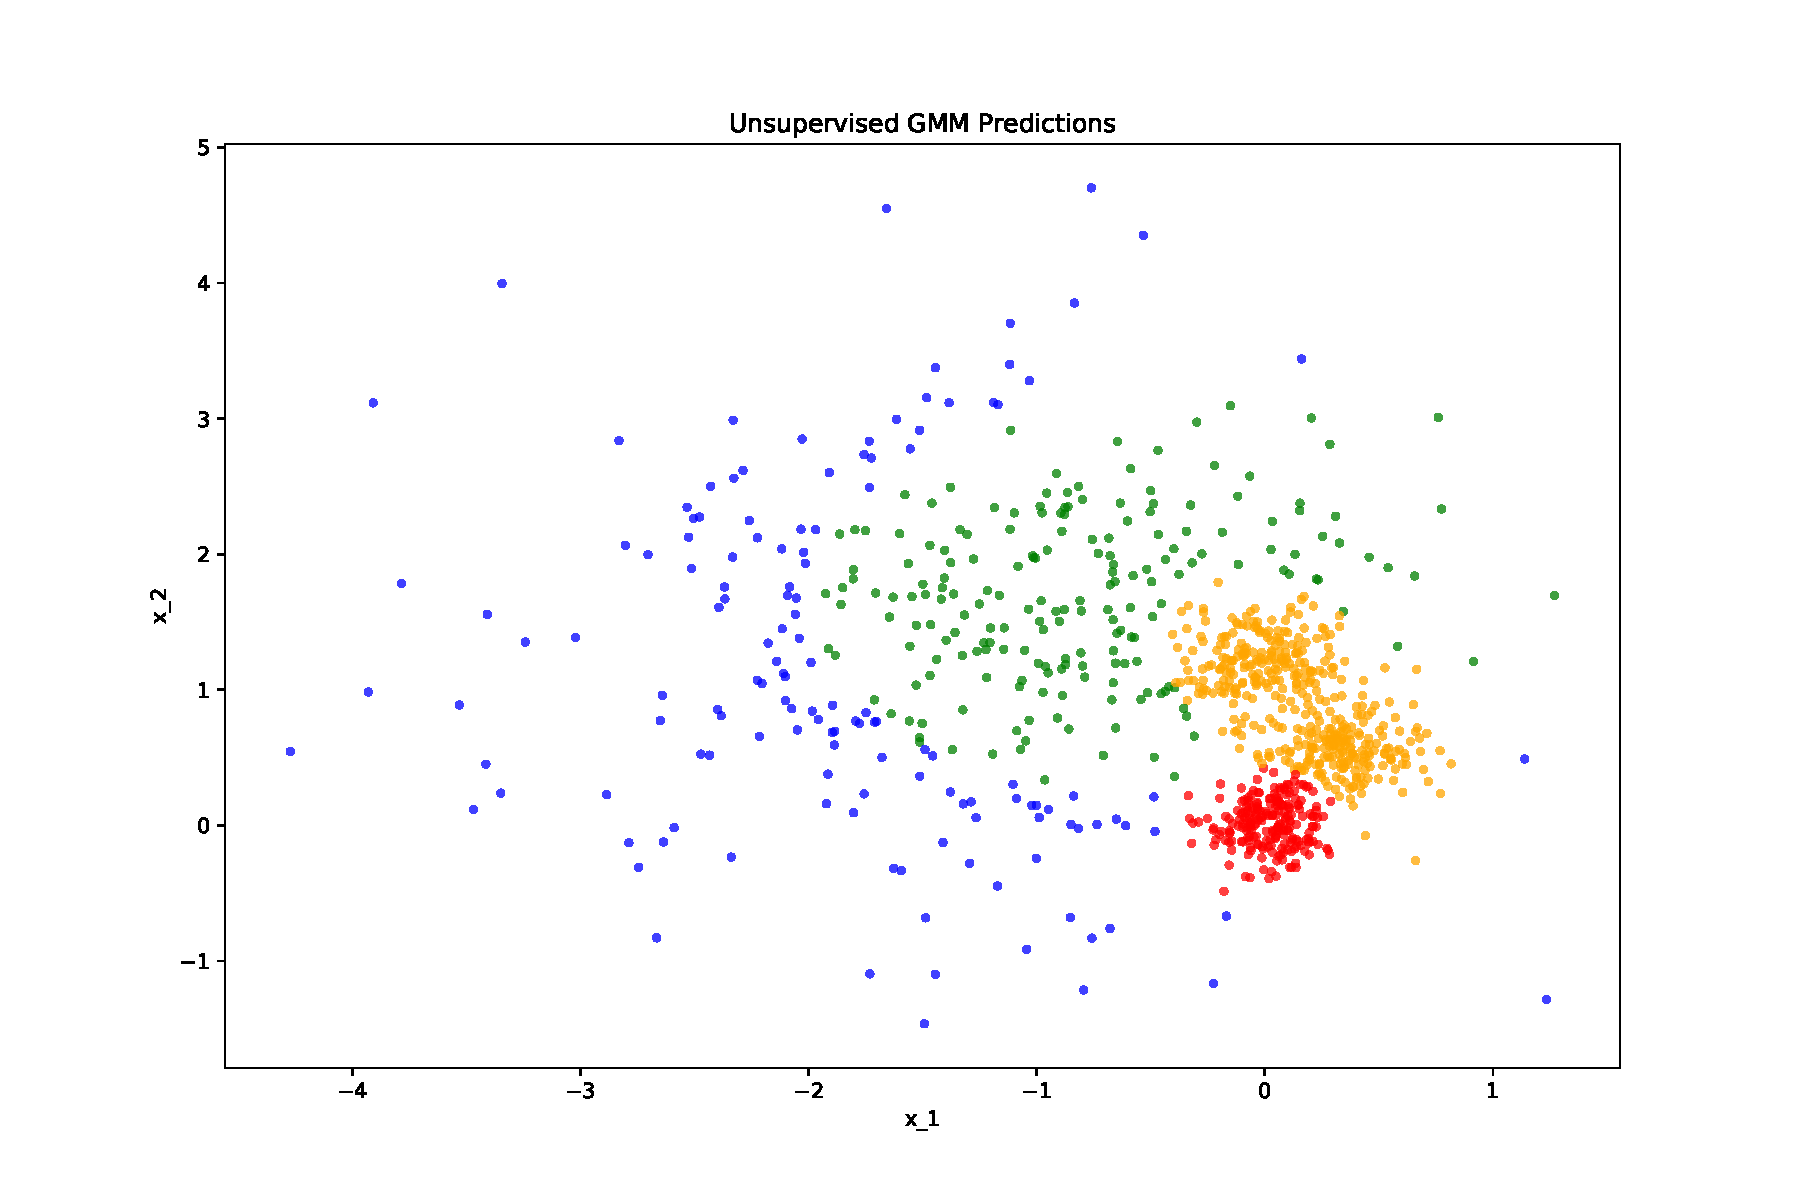
\includegraphics[width=0.3\textwidth]{semi_supervised_em/pred_0.pdf}
    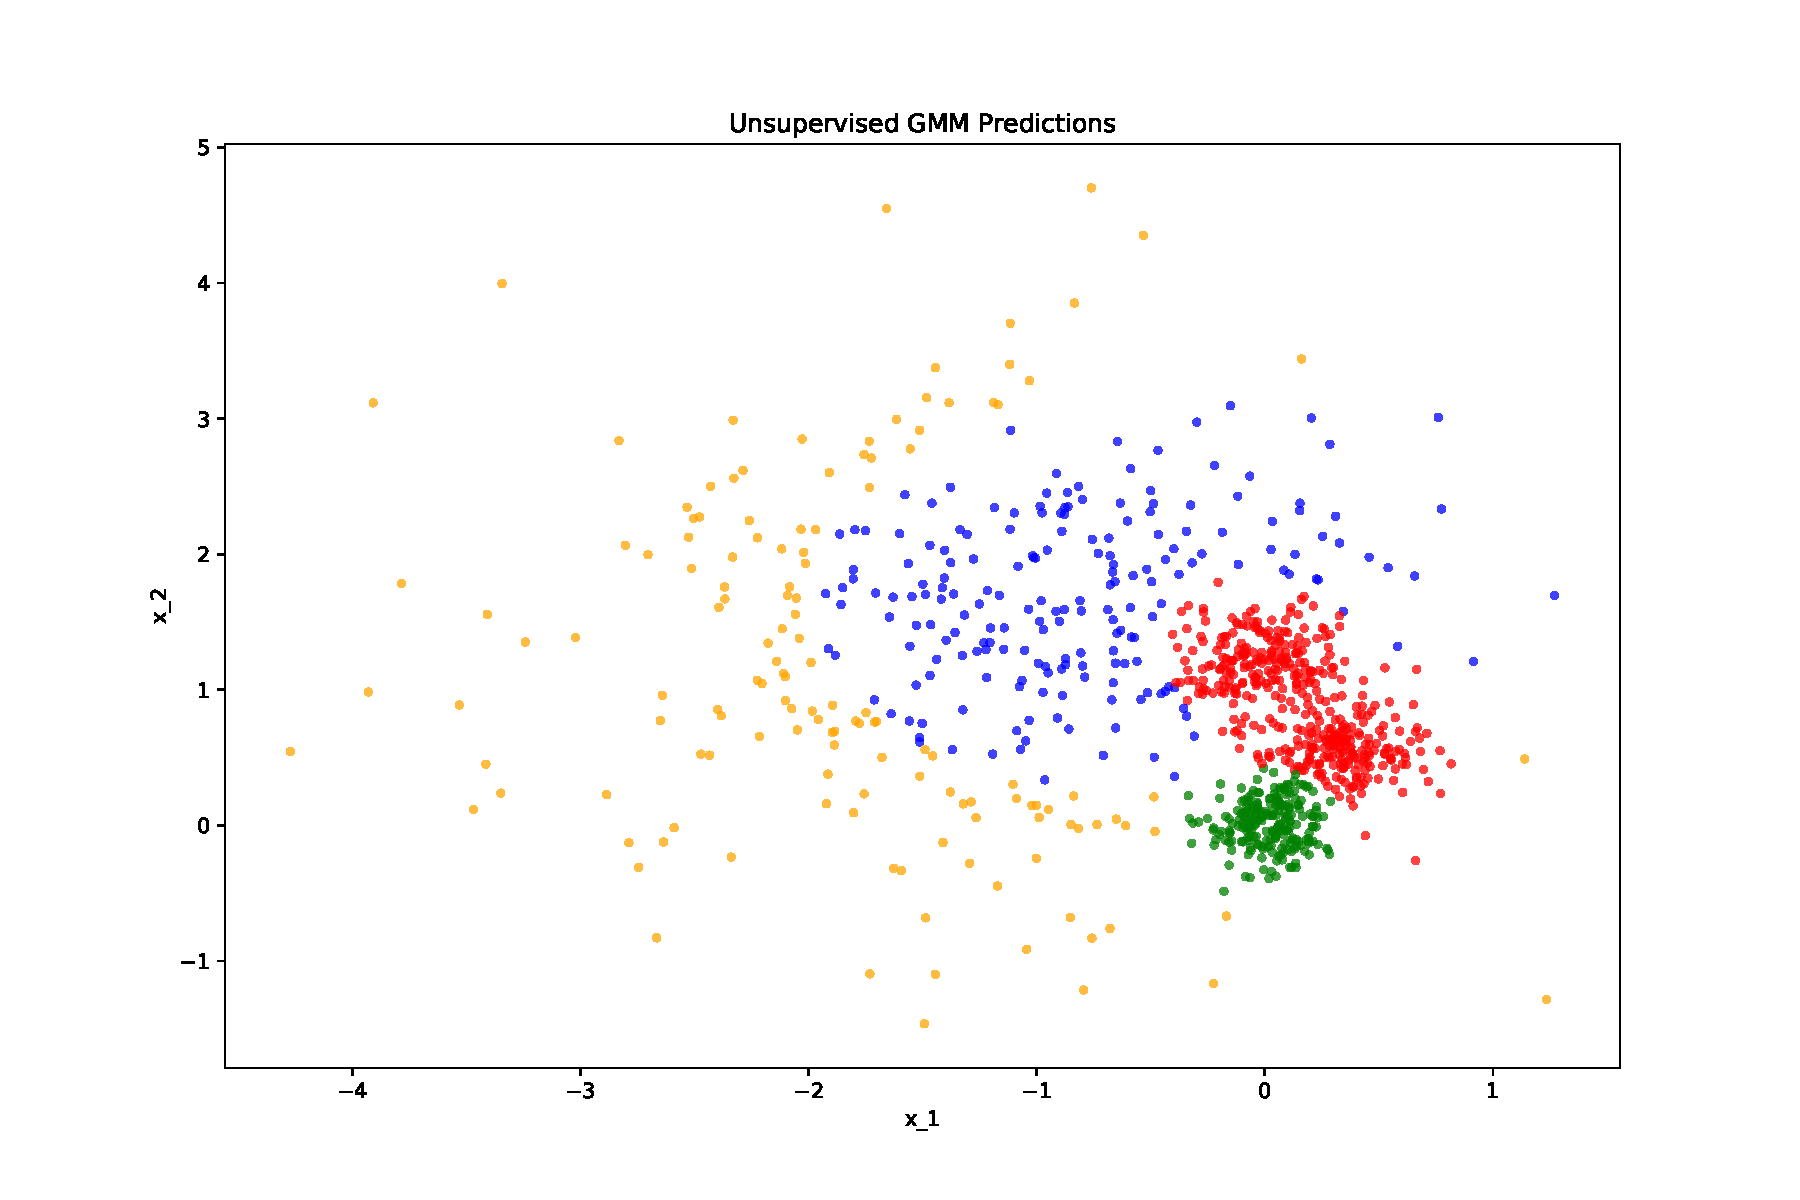
\includegraphics[width=0.3\textwidth]{semi_supervised_em/pred_1.pdf}
    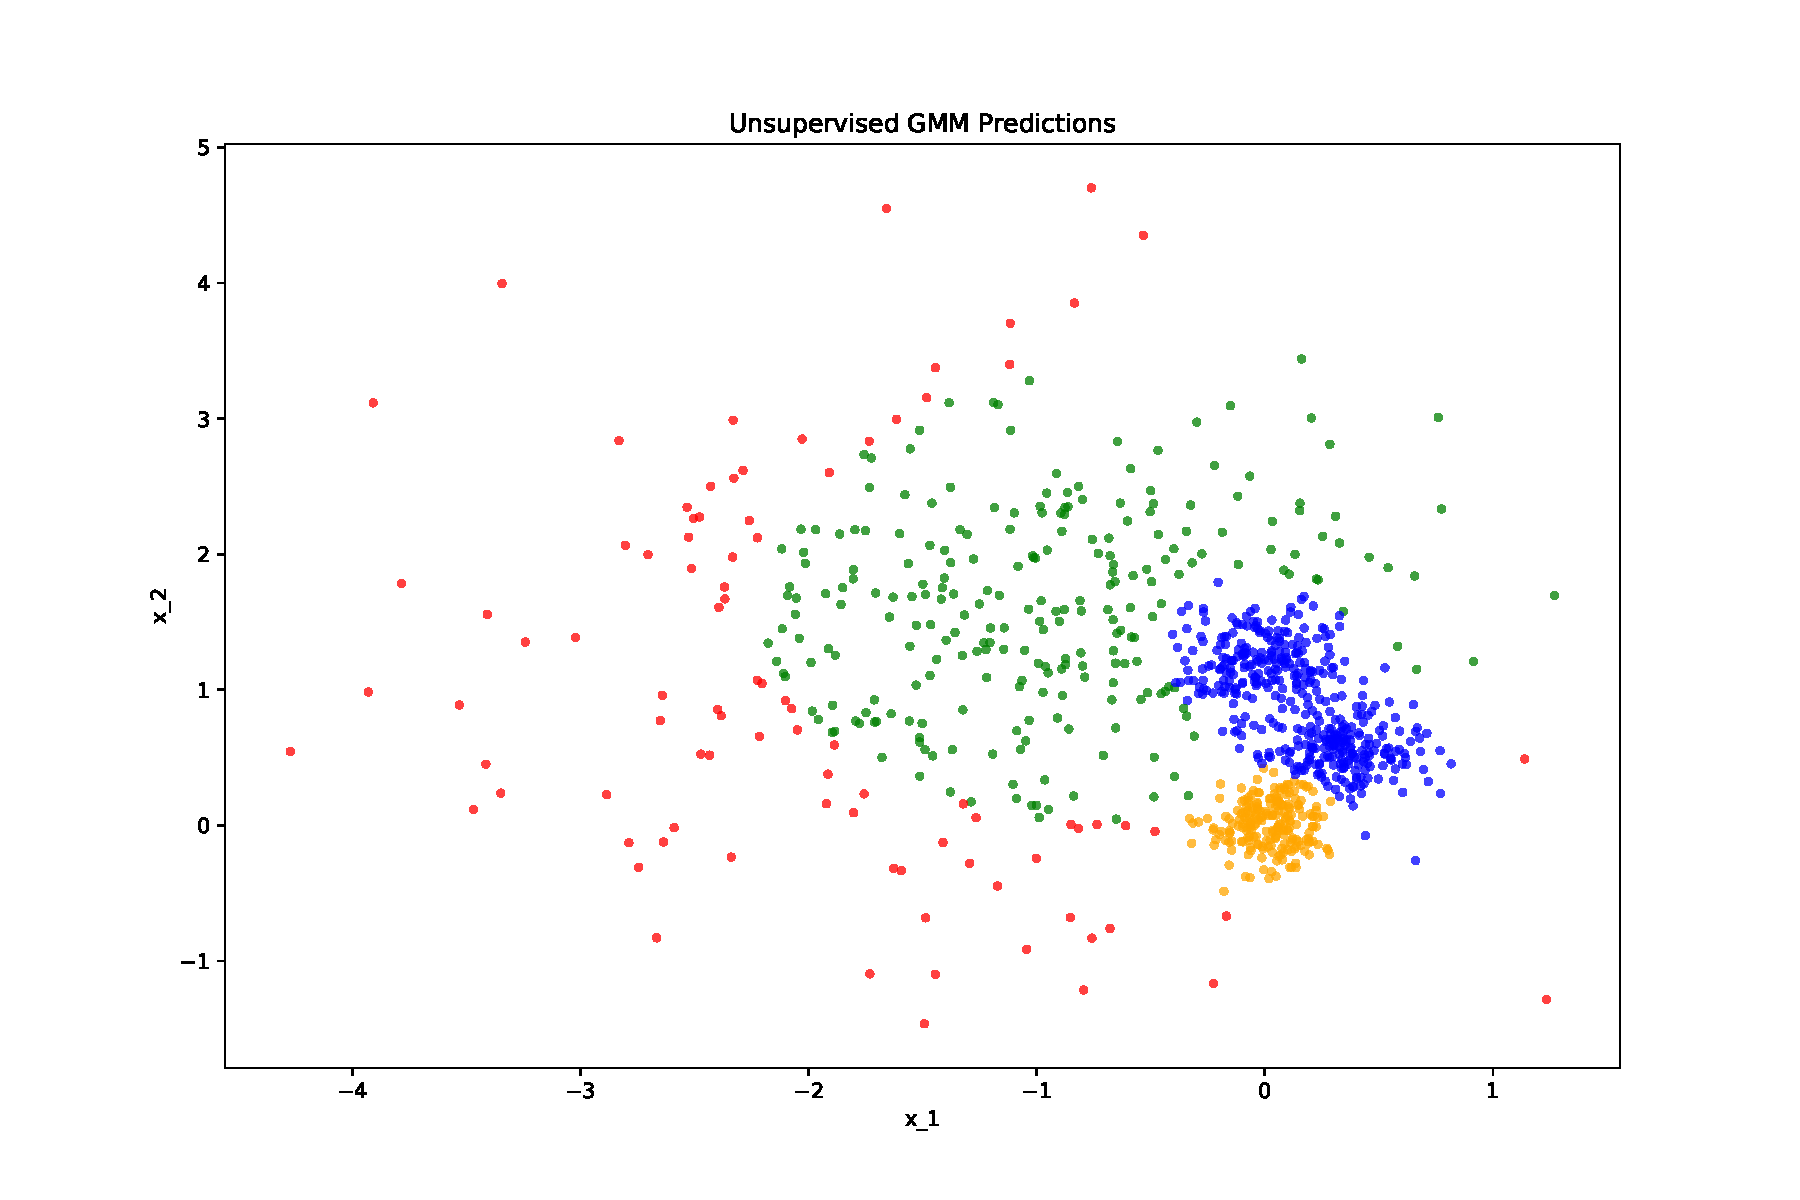
\includegraphics[width=0.3\textwidth]{semi_supervised_em/pred_2.pdf}
    \caption{Predictions made by GMM model with unsupervised EM.}
  \end{figure}

\ifnum\solutions=1 {
  \input{semi_supervised_em/04-impl-unsupervised-sol}
} \fi

  \item\subquestionpointscoding{5} \textbf{Semi-supervised EM Implementation.}
Now we will consider both the labelled and unlabelled examples (a total of $\nexp + \tilde{\nexp}$), with 5 labelled examples per cluster. We have provided starter code for splitting the dataset into matrices \texttt{x} and \texttt{x\_tilde} of unlabelled and labelled examples respectively. Add to your code in \texttt{src/semi\_supervised\_em/gmm.py} to implement the modified EM algorithm, and run it on the dataset until convergence.

To verify a correct implementation, consider creating a plot for each trial, as done in the previous sub-question.

Your plots should look similar to the following (your plots are not graded):

  \begin{figure}[H]
    \centering
    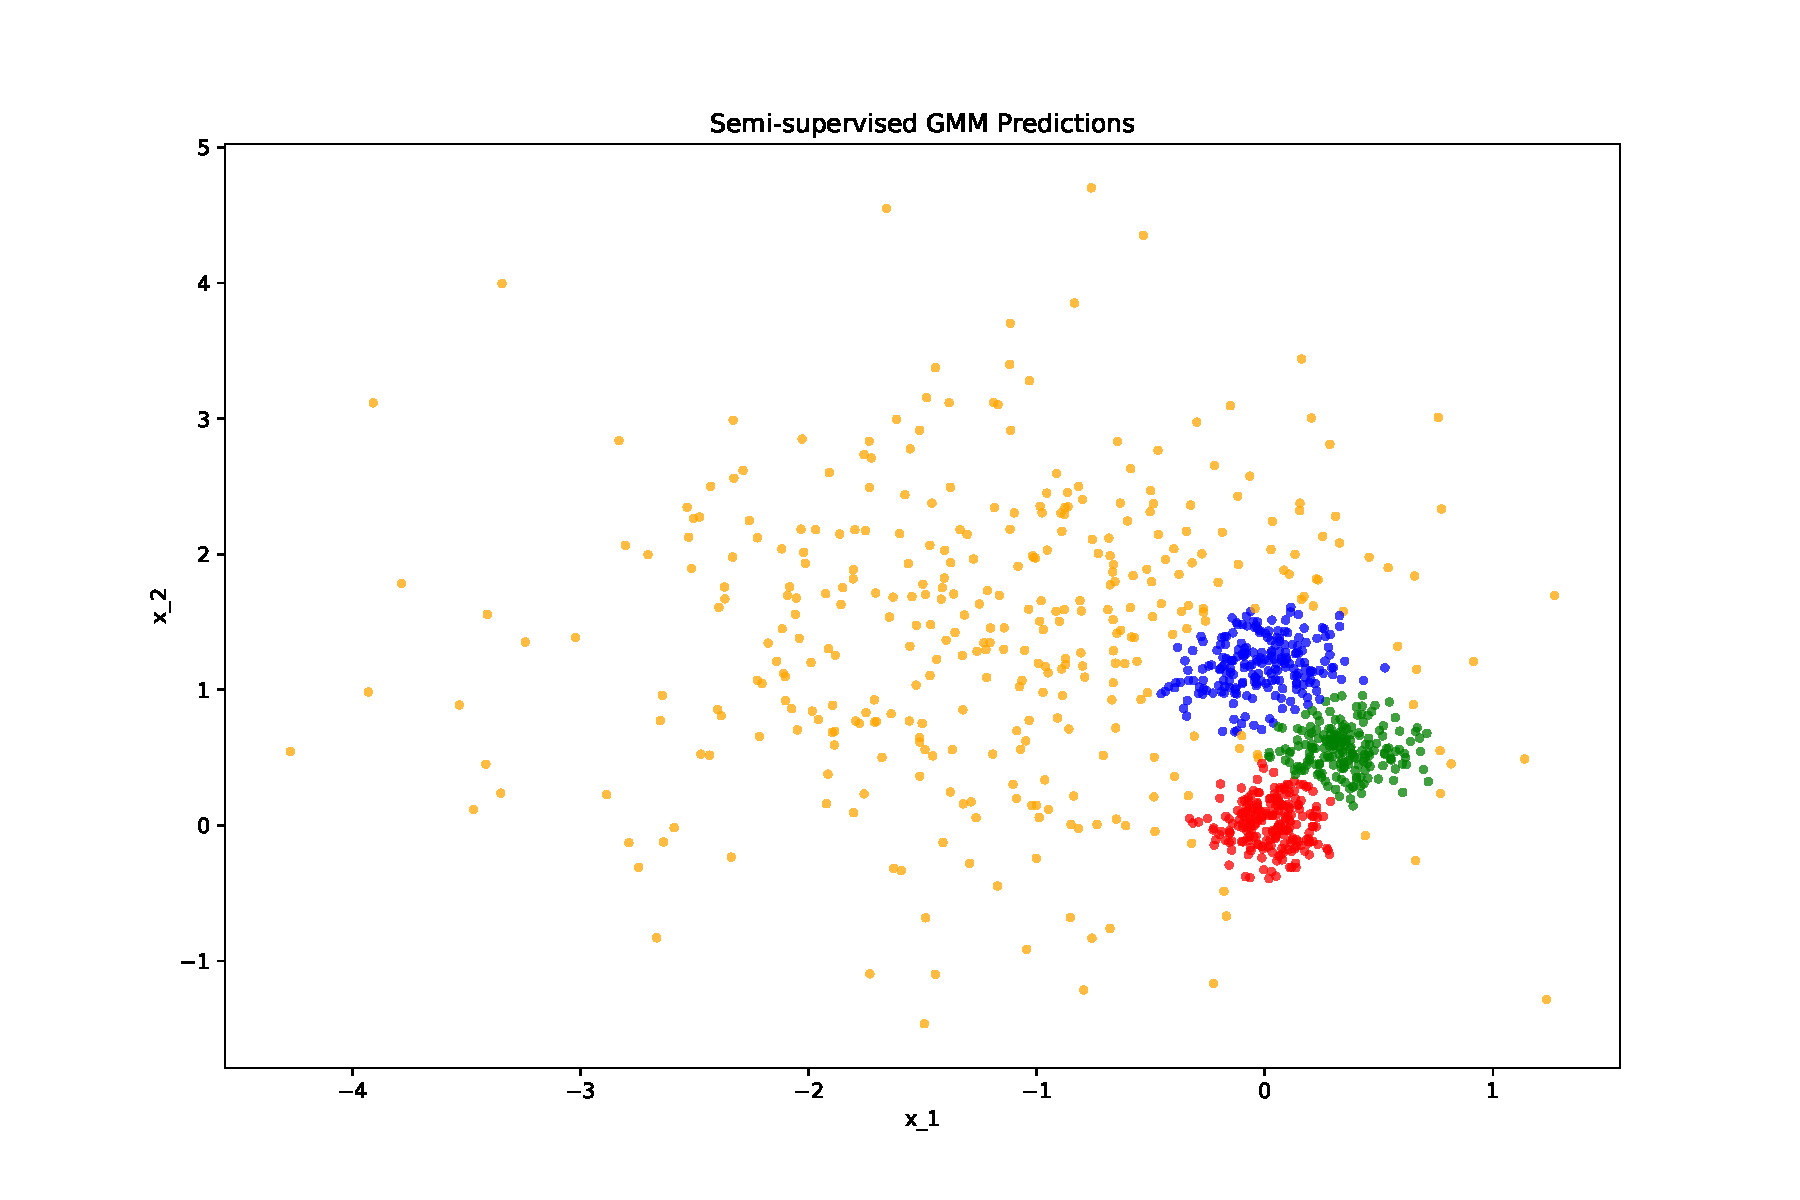
\includegraphics[width=0.3\textwidth]{semi_supervised_em/pred_ss_0.pdf}
    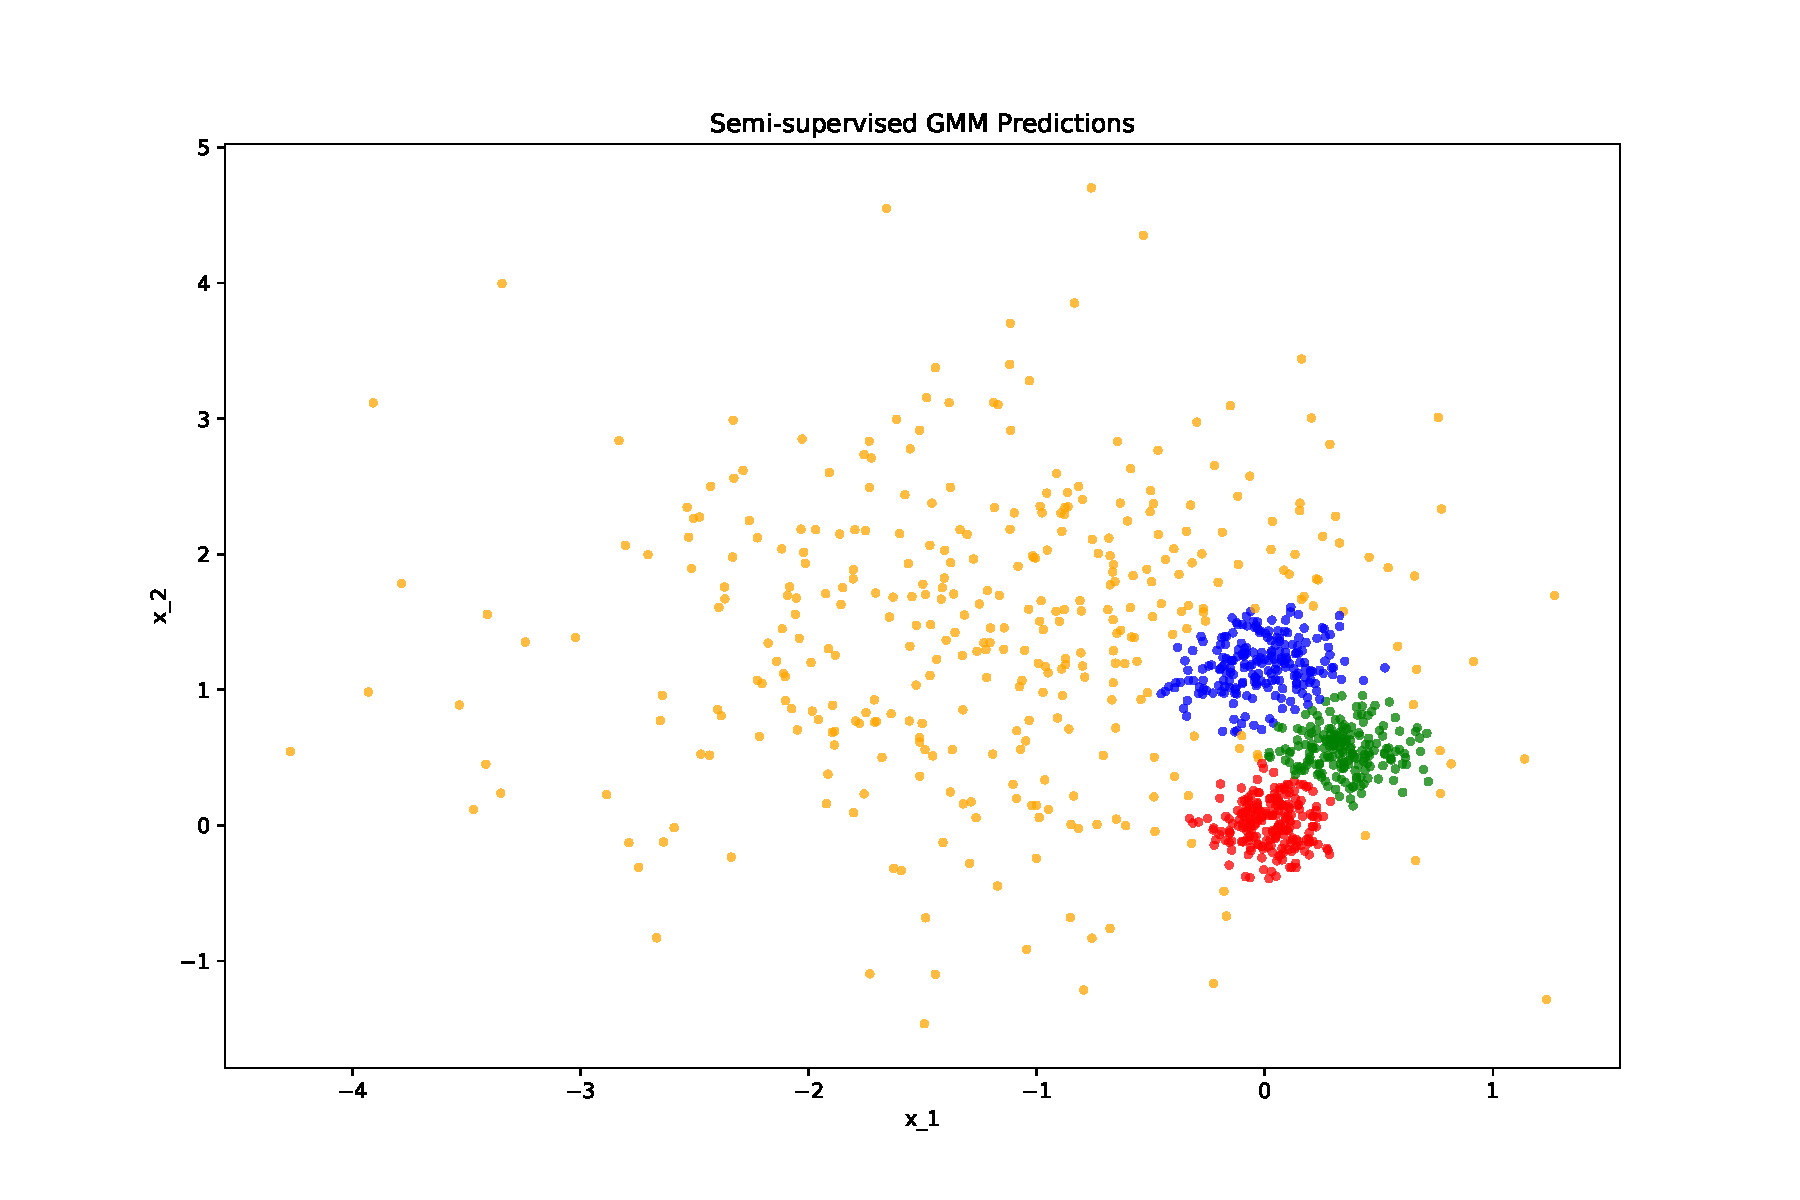
\includegraphics[width=0.3\textwidth]{semi_supervised_em/pred_ss_1.pdf}
    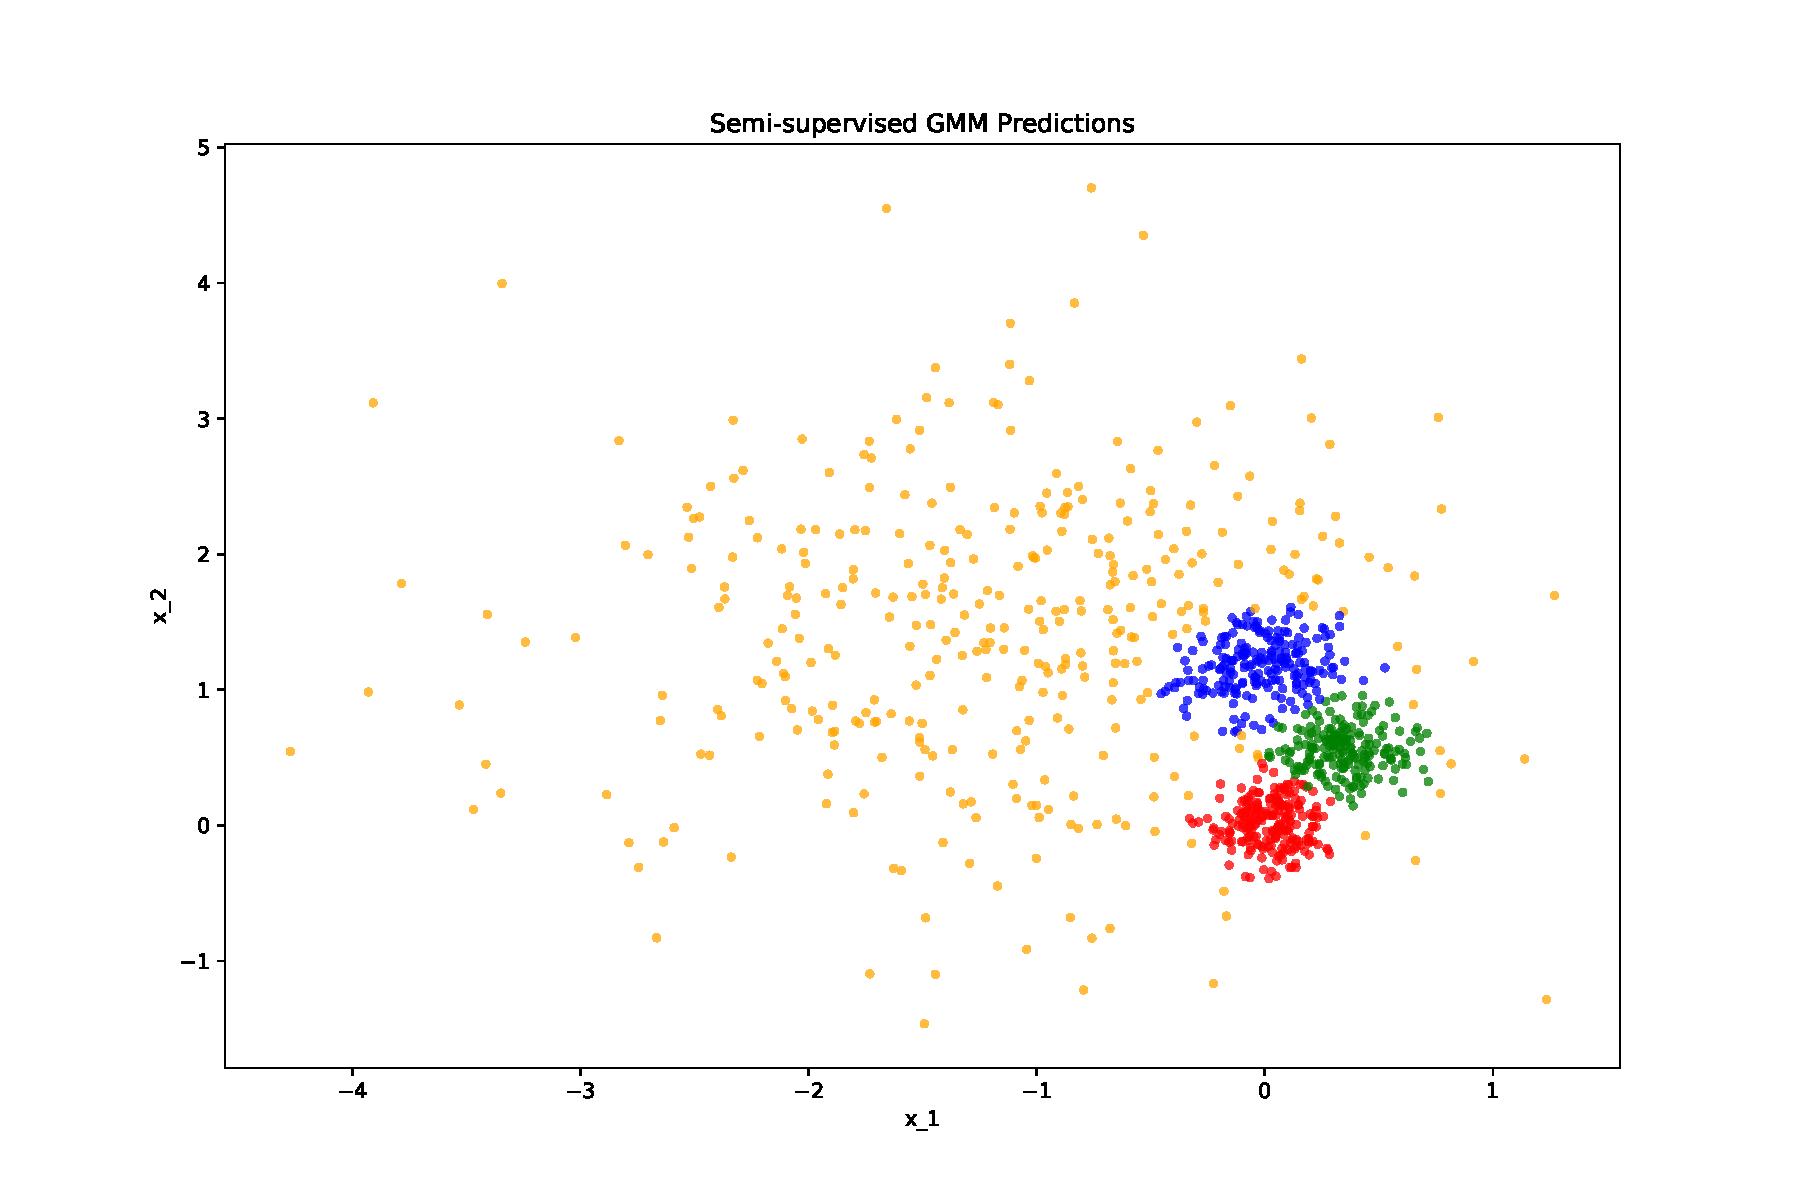
\includegraphics[width=0.3\textwidth]{semi_supervised_em/pred_ss_2.pdf}
    \caption{Predictions made by GMM model with semi-supervised EM.}
  \end{figure}

\ifnum\solutions=1 {
  \input{semi_supervised_em/05-impl-semi-supervised-sol}
} \fi

  \item\subquestionpointswritten{3} \textbf{Comparison of Unsupervised and Semi-supervised EM.}
Briefly describe the differences you saw in unsupervised \emph{vs.} semi-supervised EM for each of the following:
\begin{enumerate}[label=\roman*.]
    \item Number of iterations taken to converge.
    \item Stability (\emph{i.e.,} how much did assignments change with different random initializations?)
    \item Overall quality of assignments.
\end{enumerate}

\textbf{Note:} The dataset was sampled from a mixture of three low-variance Gaussian distributions, and a fourth, high-variance Gaussian distribution. This should be useful in determining the overall quality of the assignments that were found by the two algorithms.


\ifnum\solutions=1 {
  \input{semi_supervised_em/06-comparison-sol}
} \fi

\end{enumerate}
